% Artigo final de Trabalho de Conclusão de Curso
% Curso de Ciência da Computação — Universidade de Passo Fundo
% Autor: Igor Zanette — Matrícula: 198862
% Orientador: Prof. Rafael Rieder
%
% ESTRUTURA definida pelo orientador em 10/10/2026:
%   Introdução .................. máx. 1 página
%   Revisão de Literatura ....... máx. 2 páginas
%   Materiais e Métodos ......... com subseção do aplicativo desenvolvido
%   Resultados e Discussão ...... seção principal
%   Conclusão ................... 3 a 4 parágrafos
%
% SOBRE A CLASSE: `upf-ccc` é a mesma da proposta (docs/proposta/), por decisão do
% autor em 10/10/2026. Ela é classe de MONOGRAFIA — 12 pt, uma coluna —, então os
% limites de página acima não correspondem ao que corresponderiam num modelo de artigo
% em duas colunas. Os alvos foram convertidos para contagem de PALAVRAS, anotada no
% cabeçalho de cada arquivo de seção. Se o orientador indicar outro template, o conteúdo
% migra sem reescrita: cada seção é um arquivo isolado.

\documentclass[alpha-refs,brazilian,oneside]{upf-ccc}

%----------------------------------------------------------------
% Pacotes adicionais
%----------------------------------------------------------------
\usepackage{graphicx}
\usepackage{multirow}
\usepackage{nicefrac}
\usepackage{epstopdf}
\usepackage{chngcntr}
\counterwithout{figure}{chapter}
\counterwithout{table}{chapter}
\counterwithout{equation}{chapter}
\counterwithout{footnote}{chapter}
\usepackage{notoccite}
\usepackage{adjustbox}
\usepackage{enumitem}
\usepackage{threeparttable}
\usepackage{xcolor}
\usepackage{booktabs}

%----------------------------------------------------------------
% Marcador de pendência
%----------------------------------------------------------------
% Dado que ainda NÃO existe aparece assim, em vermelho e impossível de confundir com
% texto pronto. A regra do trabalho é que nenhum resultado seja escrito antes de ser
% medido: onde falta dado, fica o marcador dizendo o que falta e de onde virá.
% Antes de entregar: compilar e conferir que não sobrou nenhum.
\newcommand{\pendente}[1]{%
  \textcolor{red}{\textbf{[PENDENTE: #1]}}%
}

%----------------------------------------------------------------
% Ajuste de quebra de linha
%----------------------------------------------------------------
\tolerance=1000
\emergencystretch=3em
\hyphenpenalty=200
\hyphenation{
  apti-dão edá-fica frutí-feras macieira maracu-jazeiro
  mirti-leiro nogueira-pecã quivi-zeiro espe-cia-lista
  con-cor-dân-cia infe-rência reco-men-dação inter-pre-tação
  Embra-pa Comis-são fer-tili-dade adu-bação cala-gem
  pro-pri-edades microba-cias heu-rís-ticas usa-bili-dade}

%----------------------------------------------------------------
% Dados do trabalho (OBRIGATÓRIO)
%----------------------------------------------------------------
\author{Igor Zanette}

\title{SIRAS: Sistema de Interpretação e Recomendação Agronômica de Solo}
      {SIRAS: a Soil Interpretation and Agronomic Recommendation System}

\tipotrabalho{\monografia}

\orientador{Rafael Rieder}

%----------------------------------------------------------------
\begin{document}

\tableofcontents

% Resumo e abstract.
% ESTADO: rascunho. Os números citados já estão medidos, mas o resumo é a ÚLTIMA coisa a
% reescrever — ele precisa refletir o capítulo 4 fechado, inclusive usabilidade.

\chapter*{Resumo}
\addcontentsline{toc}{chapter}{RESUMO}

A interpretação de análises de solo e a derivação de recomendações de calagem e adubação
exigem conhecimento técnico e são sujeitas a erro, com consequências financeiras diretas
para o produtor. No Rio Grande do Sul e em Santa Catarina, os critérios estão
consolidados no Manual de Calagem e Adubação da CQFS-RS/SC, mas as ferramentas
computacionais disponíveis concentram-se na recomendação de correção, sem estimar a
aptidão da cultura escolhida frente às condições do solo da área; os sistemas que avaliam
aptidão, por sua vez, operam em escala regional e não se aplicam a uma análise
individual. Este trabalho apresenta o SIRAS, sistema especialista baseado em regras que
integra as duas perspectivas a partir de uma única análise de solo, cobrindo as 61
culturas e grupos de culturas para os quais o Manual publica tabelas completas de
adubação. O sistema interpreta os atributos informados, calcula a necessidade de calcário
pelo índice SMP e as doses de nitrogênio, fósforo e potássio, indica o adubo formulado
que atende à recomendação pelo procedimento do próprio Manual, e estima a aptidão edáfica
em dois cenários --- o estado atual do solo e o projetado após as correções recomendadas.
Toda saída é rastreável à regra, à tabela e à página que a produziram. A avaliação
combinou verificação automatizada, concordância com um oráculo calculado manualmente,
conformidade do módulo de aptidão frente a uma especificação aprovada antes da
implementação, e teste de usabilidade com usuários do público-alvo. Os casos com oráculo
apresentaram concordância integral, e a conformidade da aptidão foi de 100\% em classe e
em fator determinante. \pendente{acrescentar o resultado da usabilidade em uma frase}
Conclui-se que a automatização dos critérios é viável e que a integração entre
recomendação e aptidão, a partir de dados individuais de solo, representa contribuição
frente às ferramentas disponíveis para o contexto regional.

\textbf{Palavras-chave:} sistema especialista; análise de solo; calagem e adubação;
aptidão edáfica; sistemas baseados em regras.

\chapter*{Abstract}
\addcontentsline{toc}{chapter}{ABSTRACT}

Interpreting soil analyses and deriving liming and fertilization recommendations requires
technical expertise and is error-prone, with direct financial consequences for farmers.
In southern Brazil, the criteria are consolidated in the CQFS-RS/SC Liming and
Fertilization Manual, yet available software focuses on correction recommendations
without assessing the suitability of the chosen crop for the soil conditions of the
area; conversely, land suitability systems operate at a regional scale and do not apply
to an individual soil analysis. This work presents SIRAS, a rule-based expert system that
integrates both perspectives from a single soil analysis, covering the 61 crops and crop
groups for which the Manual publishes complete fertilization tables. The system
interprets the reported attributes, computes lime requirement from the SMP buffer index
along with nitrogen, phosphorus and potassium rates, indicates the compound fertilizer
that meets the recommendation following the Manual's own procedure, and estimates
\emph{edaphic} suitability under two scenarios --- the soil as it is, and as projected
after the recommended corrections. Every output is traceable to the rule, table and page
that produced it. Evaluation combined automated verification, agreement against a
manually computed oracle, conformance of the suitability module to a specification
approved before implementation, and a usability test with target users. Cases with an
oracle showed full agreement, and suitability conformance reached 100\% for both class
and limiting factor. \pendente{add the usability result in one sentence} We conclude that
automating these criteria is feasible, and that integrating recommendation and
suitability from individual soil data constitutes a contribution over the tools available
in the regional context.

\textbf{Keywords:} expert system; soil analysis; liming and fertilization; edaphic
suitability; rule-based systems.

% Introdução — alvo: máx. 1 página do template (~750 palavras)
% Compilado de docs/proposta/2_Motivacao_e_objetivos.tex, reorganizado para o artigo:
% contextualização -> problema -> justificativa -> objetivo -> contribuição.
% O que saiu da proposta: a lista de objetivos específicos (cabe em Materiais e Métodos)
% e o bloco formal de hipóteses H0/H1 (vai para a validação).

\chapter{Introdução}\label{chap:introducao}

A interpretação de análises químicas e físicas de solo é etapa essencial do
planejamento da fertilidade e do manejo das culturas agrícolas. O processo exige
conhecimento técnico e atenção rigorosa: erros de interpretação acarretam prejuízo
financeiro ao produtor, seja pelo uso desnecessário de insumos, seja pela perda de
produtividade decorrente de correção insuficiente.

A complexidade advém da multiplicidade de variáveis envolvidas --- pH, teores de
macronutrientes e micronutrientes, capacidade de troca de cátions (CTC), saturação por
bases, textura do solo, entre outras \citep{Embrapa2011, ManualCalagem2016} --- e da
necessidade de correlacioná-las com as exigências de cada cultura. No Rio Grande do Sul
e em Santa Catarina, os critérios dessa correlação estão consolidados no Manual de
Calagem e Adubação da Comissão de Química e Fertilidade do Solo
\citep{ManualCalagem2016}, cuja aplicação manual é trabalhosa e sujeita a erro: cada
recomendação exige localizar a tabela da cultura, classificar o teor na faixa correta
segundo o teor de argila ou a CTC, e compor correção com manutenção.

Ferramentas que automatizam esse processo existem e demonstram sua viabilidade. O
FertFacil, desenvolvido para RS, SC, MS e Paraguai, cobre mais de cem cultivos e é
utilizado em mais de 480 municípios gaúchos \citep{Tiecher2016}; o AdubaTec, da Embrapa
Mandioca e Fruticultura, adota arquitetura parametrizável para fruteiras tropicais
\citep{AdubaTec2021}. Ambos, porém, concentram-se na geração da recomendação de correção
e adubação, e não estimam a aptidão da cultura escolhida frente às condições do solo da
área. Em escala mais ampla, o Sistema de Avaliação da Aptidão Agrícola das Terras
\citep{EmbrapaAptidao2025} classifica o potencial produtivo com base em levantamento
pedológico regional --- abordagem inadequada à avaliação individualizada de uma área a
partir de um laudo de análise, como apontam \cite{Hofig2015}, que registram ainda a
ausência de indicação de práticas de manejo por tipo de utilização.

Constata-se, portanto, uma lacuna: há sistemas que recomendam a correção do solo e há
métodos que avaliam aptidão em escala regional, mas não há, entre as ferramentas
acessíveis ao produtor e ao técnico do RS, uma solução que integre as duas perspectivas
a partir de uma única análise de solo. É essa lacuna que o presente trabalho endereça.

A motivação é também prática. O autor acumulou experiência na assistência técnica a
produtores rurais, com contato direto com laudos e recomendações, e no atendimento
bancário a carteiras de crédito rural. Nessa última atividade observa-se que projetos
agrícolas submetidos às instituições financeiras podem apresentar inconsistências nas
recomendações técnicas, o que evidencia a necessidade de instrumentos que apoiem a
verificação dessas informações de maneira objetiva e rastreável.

Este artigo apresenta o \textbf{SIRAS} --- \textbf{S}istema de \textbf{I}nterpretação e
\textbf{R}ecomendação \textbf{A}gronômica de \textbf{S}olo ---, um sistema especialista
baseado em regras que, a partir dos dados de uma análise de solo e de uma cultura alvo,
(i)~interpreta os atributos informados segundo as faixas do Manual; (ii)~calcula a
necessidade de calcário e as doses de nitrogênio, fósforo e potássio; (iii)~indica o
adubo formulado que atende à recomendação; e (iv)~estima a \textbf{aptidão edáfica} da
cultura em dois cenários, o estado atual do solo e o estado projetado após as correções
que o próprio sistema recomendou.

O objetivo geral do trabalho foi desenvolver e avaliar o SIRAS, cobrindo as 61 culturas
e grupos de culturas para os quais o Manual publica tabelas completas de adubação.
Adota-se deliberadamente o termo \emph{aptidão edáfica}, e não \emph{aptidão agrícola}:
a estimativa restringe-se aos atributos químicos e físicos informados na análise, sem
relevo, clima, drenagem ou suscetibilidade à erosão, e empregar o termo consagrado
sugeriria equivalência com o sistema de \cite{EmbrapaAptidao2025} que não existe.

Três características distinguem a solução. A primeira é a \textbf{integração} entre
recomendação de manejo e estimativa de aptidão a partir de uma análise individual ---
o diferencial frente às ferramentas levantadas. A segunda é a \textbf{rastreabilidade}:
cada número do laudo é acompanhado da regra que o produziu e da tabela e página do
Manual de onde ela vem, o que torna o documento conferível por terceiros, requisito
relevante no contexto de análise de crédito rural. A terceira é a \textbf{separação
explícita entre norma e dado de mercado}: o que é transcrição do Manual, o que é
legislação, o que é convenção comercial e o que é ficha de fabricante ficam declarados
no próprio sistema, e não se confundem na saída.

O restante do artigo está organizado como segue. O \cref{chap:revisao} sintetiza os
conceitos e os trabalhos relacionados necessários à compreensão da solução. O
\cref{chap:metodologia} descreve os materiais, o método e a arquitetura do sistema
desenvolvido. O \cref{chap:resultados} apresenta e discute a avaliação realizada, e o
\cref{chap:conclusao} retoma o objetivo, as contribuições e as limitações.

% Revisão de Literatura — alvo: máx. 2 páginas do template (~1500 palavras)
% Seleção e síntese de docs/proposta/3_Revisao_Literatura.tex.
% O que saiu: o parágrafo de método da revisão narrativa (cabe na monografia, não no
% artigo), o detalhamento parâmetro a parâmetro da análise química, e o exemplo de IoT
% de Shahzadi, que ilustra sistema especialista em domínio distante deste.
% O que entrou: os conceitos de que o leitor precisa para entender a SOLUÇÃO — índice
% SMP, classes de disponibilidade, e o que distingue aptidão agrícola de aptidão edáfica.

\chapter{Revisão de Literatura}\label{chap:revisao}

\section{Interpretação de análise de solo e critérios do Manual RS/SC}

A análise de solo é o principal instrumento de diagnóstico da fertilidade e de
planejamento do manejo nutricional \citep{Embrapa2011}. Dela resultam o pH em água, que
condiciona a disponibilidade da maioria dos nutrientes; os teores de fósforo disponível
e de potássio, cálcio e magnésio trocáveis; o alumínio trocável, associado à toxidez em
solos ácidos; a CTC, que expressa a capacidade de reter e fornecer nutrientes; e a
saturação por bases \citep{Embrapa2011, ManualCalagem2016}. A textura, dada pela
proporção de areia, silte e argila, é o atributo físico central da interpretação, por
influenciar a CTC, a retenção de água e a resposta à calagem; o teor de matéria orgânica
contribui para a CTC efetiva e para a disponibilidade de nitrogênio \citep{Santos2003}.
A interpretação exige comparar cada valor a faixas de referência estabelecidas por
parâmetro, tipo de solo e cultura \citep{EmbrapaDoc206}.

Para o Rio Grande do Sul e Santa Catarina, essas faixas e os procedimentos de cálculo
estão consolidados no Manual de Calagem e Adubação da CQFS-RS/SC
\citep{ManualCalagem2016}, referência técnica adotada neste trabalho como fonte única.
Três mecanismos do Manual são indispensáveis à compreensão da solução.

O primeiro é o \textbf{índice SMP}. A necessidade de calcário é estimada
preferencialmente por esse índice tampão, e não pela saturação por bases: a Tabela 5.2
do Manual converte o valor de SMP da amostra na quantidade de corretivo de PRNT 100\%
necessária para elevar o pH da camada de 0 a 20~cm a 5,5, 6,0 ou 6,5. O método da
saturação por bases existe como alternativa, mas a primeira calagem usa SMP. A dose
tabelada é depois convertida para o corretivo real pela razão entre 100 e o PRNT do
produto.

O segundo é a distinção entre \textbf{pH de referência} e \textbf{critério de disparo}.
A Tabela 5.1 atribui um pH de referência a cada cultura, mas não é ele que determina
quando aplicar calcário: o disparo e o pH alvo vêm das Tabelas 5.3 a 5.7, por grupo de
cultura, e frequentemente divergem do pH de referência. As culturas de grãos, por
exemplo, têm pH de referência 6,0 e só recebem calcário quando o pH está abaixo de 5,5,
com dose calculada para 6,0. Tratar o pH de referência como gatilho é erro comum e
produz recomendação equivocada.

O terceiro é a \textbf{interpretação por classes de disponibilidade} --- muito baixo,
baixo, médio, alto e muito alto. A classe do fósforo depende da classe de teor de argila
do solo, e a do potássio depende da CTC a pH 7,0; cada cultura pertence a um grupo de
exigência que determina qual coluna da tabela se aplica. A dose recomendada combina uma
parcela de correção, função da classe, com uma parcela de manutenção, função da
expectativa de rendimento. Leguminosas como soja, ervilhaca e tremoço não recebem
adubação nitrogenada, em razão da fixação biológica de nitrogênio.

O Manual trata ainda da conversão da recomendação em produto comercial
(\S8.3, p.~310--311): a fórmula adequada é múltipla da proporção da recomendação e,
quando não há fórmula exata, a dose se ajusta ao nutriente mais deficiente no solo, com
o saldo de nitrogênio aplicado em cobertura. Esse procedimento é a base do módulo de
indicação de adubo descrito no \cref{chap:metodologia}.

\section{Aptidão agrícola e aptidão edáfica}

A avaliação da aptidão agrícola das terras classifica áreas segundo seu potencial para
diferentes usos, considerando as limitações impostas pelo solo e pelo relevo sob
distintos níveis tecnológicos. O sistema de referência no Brasil classifica as terras em
seis grupos a partir de cinco fatores de limitação --- deficiência de fertilidade,
deficiência hídrica, excesso de água, suscetibilidade à erosão e impedimentos à
mecanização \citep{EmbrapaAptidao2025}; sua formulação metodológica remonta a
\cite{RamalhoFilhoBeek1995}.

\cite{Hofig2015}, em estudo no município de Cerro Grande do Sul/RS, apontam que esse
sistema é mais adequado a análises de âmbito regional, não indica práticas de manejo por
tipo de utilização e não foi projetado para a avaliação individualizada de propriedades
a partir de dados de análise de solo, exigindo adaptações para o planejamento
conservacionista em escala de propriedade.

Uma abordagem alternativa estima a aptidão a partir dos próprios parâmetros da análise,
cruzados com as exigências agronômicas da cultura, sem considerar relevo e clima. É o
que este trabalho denomina \textbf{aptidão edáfica}: estimativa delimitada às condições
químicas e físicas do solo para uma cultura específica, adequada à avaliação de uma área
a partir de um laudo. A distinção terminológica é deliberada e necessária --- o próprio
Manual \citep[Cap.~2, p.~23]{ManualCalagem2016} registra que a aptidão agrícola depende
de fatores de ambiente que uma análise de solo não informa, de modo que empregar o termo
consagrado para o subconjunto edáfico sugeriria uma equivalência inexistente.

\section{Sistemas especialistas baseados em regras}

Sistemas especialistas são programas que reproduzem o raciocínio de um especialista
humano em domínio restrito, apoiando diagnóstico e recomendação \citep{SantosEtAl1994}.
Compõem-se de três elementos: a \textbf{base de conhecimento}, que armazena fatos,
regras e heurísticas; o \textbf{motor de inferência}, que aplica as regras aos dados de
entrada para derivar conclusões; e a \textbf{interface} com o usuário.

Os sistemas baseados em regras do tipo SE-ENTÃO são a abordagem mais difundida para
representar conhecimento agronômico: cada regra expressa um fragmento do conhecimento
especialista na forma \textit{SE} <condição> \textit{ENTÃO} <conclusão>, e o motor
percorre a base identificando quais condições os dados satisfazem \citep{Lanzer2010}.

\cite{Lanzer2010} desenvolveu sistema especialista baseado em regras para classificação
do uso e manejo das terras, com representação hierárquica do conhecimento --- indicada
para sistemas de classificação --- compatível com o sistema brasileiro. O autor observa
que a introspecção facilita o desenvolvimento nos estágios iniciais quando as
informações para a definição dos estados já estão presentes nos próprios sistemas de
classificação, que é exatamente o caso do Manual de Calagem e Adubação: suas tabelas são
uma base de regras já formalizada, que o sistema transcreve em vez de inferir.

Essa propriedade sustenta a escolha arquitetural deste trabalho. Em domínio cujo
conhecimento está publicado em forma tabular e normativa, um motor de regras explícito
oferece algo que métodos estatísticos ou de aprendizado de máquina não ofereceriam:
cada saída é rastreável à regra e à tabela que a produziram. Em um documento que pode
instruir projeto de crédito rural, a auditabilidade não é conveniência, é requisito.

\section{Trabalhos relacionados}

O \textbf{FertFacil} \citep{Tiecher2016} é sistema online e gratuito que estima a
necessidade de adubação e calagem para os principais cultivos do RS, SC, MS e Paraguai,
com base nos critérios do Manual. Cobre mais de cem cultivos, é ferramenta de escolha da
Emater/RS e é usado em mais de 480 municípios. Sua limitação, para o escopo aqui
tratado, é a ausência de estimativa de aptidão integrada à recomendação.

O \textbf{AdubaTec} \citep{AdubaTec2021}, da Embrapa Mandioca e Fruticultura em parceria
com a UFRB, recomenda calagem e adubação para mandioca e fruteiras tropicais, com
arquitetura parametrizável que permite incorporar culturas sem alterar o código-fonte.
Baseia-se em manuais voltados ao Nordeste, não cobre os critérios do Manual RS/SC e
tampouco estima aptidão a partir da análise individual.

O \textbf{Sistema de Avaliação da Aptidão Agrícola das Terras}
\citep{EmbrapaAptidao2025} é a referência para classificação do potencial produtivo das
terras brasileiras, voltado a levantamentos regionais em escala exploratória e baseado
em mapeamento pedológico. Sua escala o torna inadequado à avaliação individualizada de
uma propriedade a partir de análise de solo \citep{Hofig2015}.

Do levantamento conclui-se que os sistemas disponíveis tratam, separadamente, da
recomendação de manejo ou da avaliação de aptidão em escala regional. Nenhum integra as
duas perspectivas a partir de uma análise individual de solo com cobertura para o Manual
RS/SC --- lacuna que motiva a solução descrita a seguir.

% Materiais e Métodos
% Base: docs/proposta/4_Metodologia.tex, com os verbos no PASSADO e só o que foi
% efetivamente realizado. Acrescenta a subseção 3.4, do aplicativo desenvolvido, que a
% proposta não tinha. Retirado da proposta: alternativas tecnológicas descartadas, o
% cronograma e os resultados esperados.
%
% ESTA SEÇÃO ESTÁ COMPLETA — descreve o que foi feito, e tudo o que ela afirma já existe.

\chapter{Materiais e Métodos}\label{chap:metodologia}

\section{Caracterização da pesquisa}

A pesquisa caracteriza-se como descritiva e aplicada: estrutura um conjunto de critérios
técnicos já consolidados na literatura agronômica e aplica esse conhecimento na
construção e na avaliação de um artefato computacional \citep{Wazlawick2014}. Quanto ao
estilo de pesquisa em Computação, enquadra-se na apresentação de um produto.

\cite{Wazlawick2014} adverte que esse estilo exige cautela, pois a simples demonstração
de funcionamento tem baixa aceitação científica: é preciso comparar o que foi construído
com alguma referência. Por isso a avaliação não se limitou à demonstração. As saídas
foram confrontadas com um oráculo técnico --- os valores obtidos pela aplicação manual e
independente dos critérios do Manual \citep{ManualCalagem2016} --- e o sistema foi
posicionado frente às ferramentas discutidas no \cref{chap:revisao}.

\section{Escopo e fonte de conhecimento}

O escopo abrange as \textbf{61 culturas e grupos de culturas} para as quais o Manual
publica tabelas completas de adubação, organizadas em seis grupos: 21 de grãos, 18
hortaliças, 2 tubérculos, 17 frutíferas, erva-mate e 2 outras culturas comerciais
(cana-de-açúcar e tabaco). A contagem segue a organização do próprio Manual, em que
culturas que compartilham tabela --- melancia e melão, por exemplo --- contam como uma
entrada. Ficaram fora o arroz irrigado por alagamento, a mandioca, as espécies
florestais tolerantes à acidez e os grupos de forrageiras, palmeiras, medicinais e
ornamentais.

A \textbf{fonte técnica é única}: o Manual de Calagem e Adubação para os estados do RS e
de SC, 11\textsuperscript{a} edição \citep{ManualCalagem2016}. A base de conhecimento foi
transcrita manualmente pelo autor a partir da publicação, e a rastreabilidade de cada
tabela para o arquivo correspondente foi registrada em documento próprio do repositório.

\subsection{Controle sobre a transcrição}

A transcrição a partir do PDF revelou uma ameaça concreta à validade que exigiu controle
explícito. O PDF do Manual \textbf{não contém o caractere \textquotesingle$\leq$\textquotesingle{} na
camada de texto}: ele é desenhado como imagem embutida de aproximadamente
6~$\times$~6~pt, que nenhuma ferramenta de extração recupera. O comportamento é
inconsistente entre páginas --- ora o símbolo desaparece, ora é devolvido como sinal de
igualdade ---, de modo que um valor exato torna-se indistinguível de um valor com
qualificador.

O procedimento adotado combinou quatro controles: extração automática do texto;
detecção programática dos glifos ausentes como objetos de imagem, filtrados por tamanho,
e sua reinserção na posição correta; conferência visual de páginas rasterizadas por
amostragem e em toda célula de qualificador duvidoso; e testes automatizados de
invariantes sobre as tabelas resultantes, como a monotonicidade das doses por classe de
teor.

O mesmo artefato explica uma decisão de leitura registrada no trabalho: notas do Manual
que condicionam exceções a teores de cálcio e magnésio aparecem no texto extraído com
sinal de igualdade, e foram lidas como limites mínimos. A leitura sustenta-se em cinco
evidências convergentes, entre elas o fato de o operador \textquotesingle$<$\textquotesingle{}
da mesma frase sobreviver à extração --- o que localiza a perda nos glifos de
desigualdade não estrita --- e o próprio Anexo~1 do Manual aplicar a exceção como
limiar em exemplo resolvido.

Como controle adicional, os grupos de exigência de fósforo e potássio de cada cultura
foram transcritos \textbf{três vezes}, em momentos e por caminhos distintos, e as três
transcrições concordam integralmente. Um teste automatizado mantém essa concordância
travada. Cabe a ressalva, porém, de que isso é evidência de \emph{correção da
transcrição}, e não de correção agronômica dos critérios.

\section{Tecnologia e arquitetura}

O sistema foi implementado em \textbf{Python 3.12} com \textbf{Flask} para a camada web.
A base de conhecimento ficou em arquivos \textbf{JSON} validados por \textit{JSON
Schema}, carregados em tempo de execução. O sistema roda localmente, sem banco de dados,
sem autenticação e sem chamada de rede.

Duas decisões de arquitetura merecem registro. A primeira: o motor de inferência foi
escrito em \textbf{Python puro}, sem biblioteca externa de sistemas especialistas. A
decisão é metodológica --- um motor de terceiros introduziria uma camada de resolução de
conflitos cujo comportamento precisaria ser, ele próprio, verificado, enquanto o objetivo
é que cada decisão seja auditável linha a linha. A segunda: os módulos de domínio e de
motor \textbf{não importam Flask}, de modo que o núcleo é executável e testável por
linha de comando, independentemente da interface.

A \cref{fig:arquitetura} resume as camadas e a fronteira entre elas.

A arquitetura separa quatro camadas: \texttt{dominio}, com as entidades;
\texttt{conhecimento}, com o carregamento e a validação da base; \texttt{motor}, com as
regras; e \texttt{relatorio} e \texttt{web}, com a apresentação. O motor expõe um
\textbf{ponto de entrada único}, a função \texttt{gerar\_laudo}, pura e determinística:
as mesmas entradas produzem sempre o mesmo laudo e a mesma trilha.


\begin{figure}[htb]
\centering
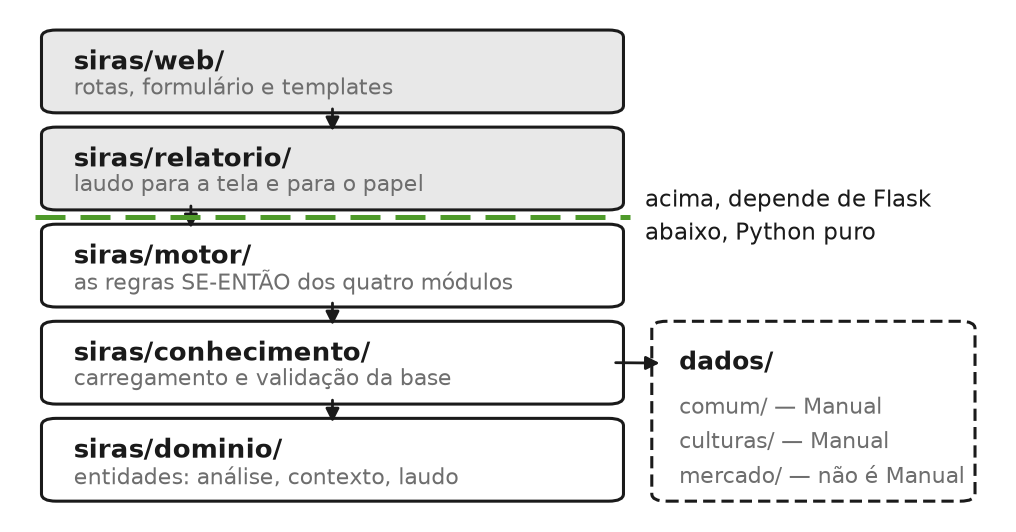
\includegraphics[width=0.95\textwidth]{fig/f1-arquitetura}
\caption{Camadas do SIRAS e a fronteira do Flask. O motor e o domínio não dependem da camada web, o que permite executá-los e testá-los por linha de comando, independentemente da interface.}
\label{fig:arquitetura}
\end{figure}

\subsection{Separação entre norma e dado de mercado}

Duas funcionalidades exigiram dados que o Manual não publica: a indicação de adubo
formulado e a caracterização de corretivos comerciais. Esses dados foram mantidos em
diretório separado da transcrição do Manual, e cada bloco declara a própria fonte e o
próprio estatuto --- lei vigente, convenção comercial herdada de norma revogada,
orientação do Manual ou ficha de fabricante.

A distinção não é formalidade de organização de arquivos. As faixas comerciais de PRNT
(A a D) e a classificação de corretivos por teor de óxido de magnésio, por exemplo, são
frequentemente apresentadas como exigência legal, mas têm origem em portaria revogada;
a norma vigente \citep{BrasilIN35_2006} fixa garantias mínimas e fatores de reatividade,
e não contém essas faixas. No sistema, elas estão rotuladas como convenção comercial histórica, e não
como norma.

\section{O aplicativo desenvolvido}\label{sec:aplicativo}

\subsection{Fluxo de uso}

O fluxo tem três telas. Na primeira, a pessoa escolhe entre os seis grupos e as 61
culturas. Na segunda, informa os dados da análise de solo; as variáveis condicionais que
cada cultura exige --- fase do pomar, ciclo da cana, tipo de tabaco, programa da
erva-mate --- aparecem por divulgação progressiva, lidas da base, de modo que a tela
nunca oferece uma opção que o motor recusaria. Enquanto a pessoa digita, um painel de
leitura ao vivo mostra em que classe cada teor caiu. Na terceira, o laudo.

A análise pode cobrir \textbf{vários talhões} num documento único, repetindo a análise
de solo por talhão e compartilhando cultura, manejo e corretivo. A área é opcional; se
informada para todos os talhões, o laudo acrescenta a quantidade total a comprar.


\begin{figure}[htb]
\centering
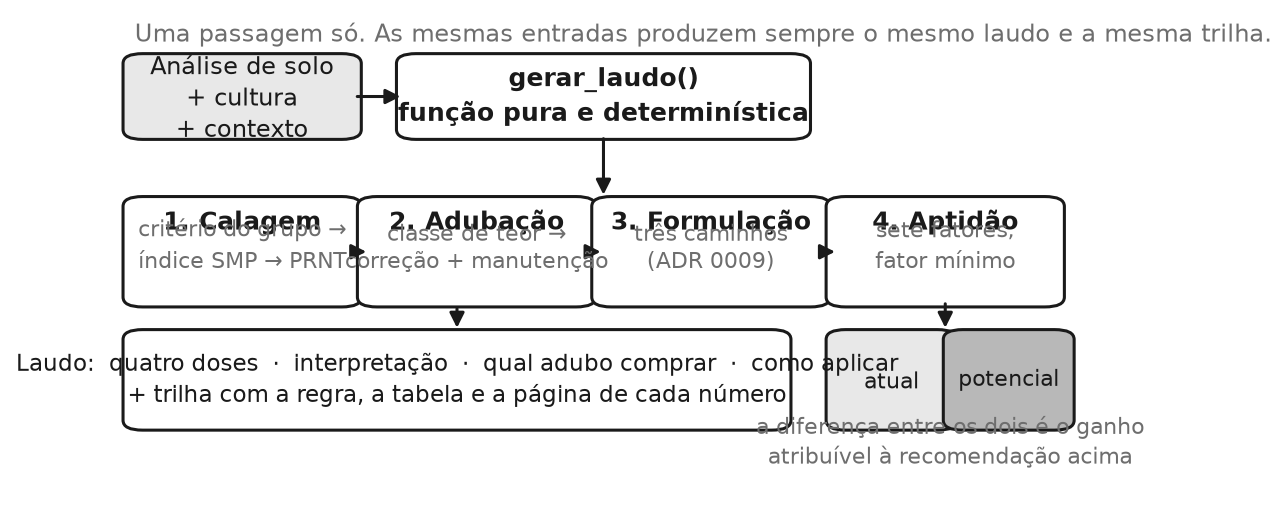
\includegraphics[width=0.95\textwidth]{fig/f2-fluxo}
\caption{Da análise de solo ao laudo, em uma passagem. A função \texttt{gerar\_laudo} é o ponto de entrada único e é determinística; os dois cenários de aptidão saem sempre juntos, porque é a diferença entre eles que quantifica o ganho atribuível à recomendação emitida.}
\label{fig:fluxo}
\end{figure}

\subsection{Módulos de recomendação}

O \textbf{módulo de calagem} resolve o critério aplicável à cultura e ao sistema de
manejo, consulta o índice SMP na Tabela 5.2 para o pH alvo do critério e converte a dose
pelo PRNT do corretivo informado. Trata os casos especiais do Manual: plantio direto
consolidado, em que a dose é um quarto da indicada para pH 6,0, aplicada em superfície e
limitada a 5~t/ha; solos de baixo poder tampão, em que equações polinomiais substituem a
tabela; e as culturas sem pH de referência, cuja calagem se decide por saturação por
bases.


\begin{figure}[htb]
\centering
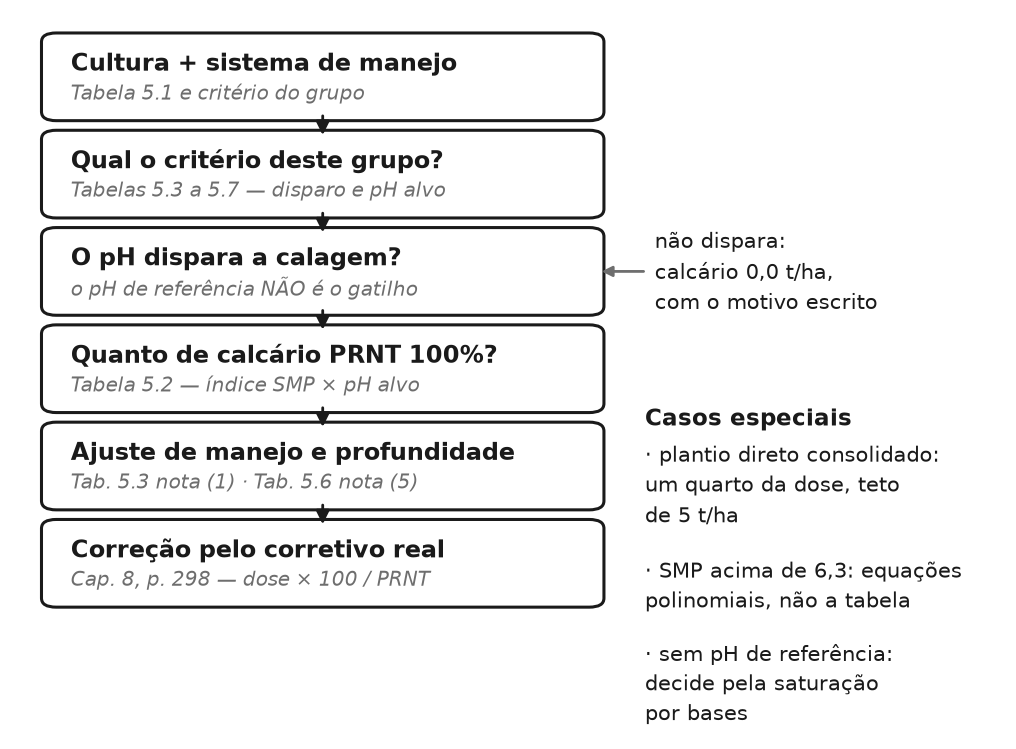
\includegraphics[width=0.88\textwidth]{fig/f3-calagem}
\caption{Decisão da dose de calcário, com a fonte de cada passo. A distinção entre o pH de referência e o critério de disparo é o ponto em que a aplicação manual do Manual mais erra.}
\label{fig:calagem}
\end{figure}

O \textbf{módulo de adubação} classifica o fósforo pela classe de teor de argila e o
potássio pela CTC a pH 7,0, segundo o grupo de exigência da cultura, e compõe as doses
de correção e manutenção. As culturas de grãos têm caminho próprio, por serem a exceção
do Manual --- publicam correção e manutenção em separado, com algoritmo por cultivo ---,
enquanto os outros cinco grupos compartilham um despacho parametrizado pelas variáveis
condicionais que cada um exige.

O \textbf{módulo de indicação de adubo formulado} converte a recomendação em produto,
pelo procedimento do Manual (\S8.3, p.~311): a dose da fórmula ancora-se no nutriente
mais deficiente no solo, que passa a ser atendido exatamente; o que faltar do outro é
completado com fertilizante simples, segundo as garantias da Tabela 8.4 --- hoje
atualizadas pela \cite{BrasilIN39_2018} ---; e o saldo de nitrogênio vai para cobertura. Entre as fórmulas do catálogo, a escolhida é a de menor
desvio relativo frente à recomendação, com desempate pela mais concentrada. O catálogo
de fórmulas é dado de mercado, declarado como tal no laudo, e o ranking é
\textbf{nutricional}: o Manual recomenda escolher pelo menor custo por unidade de NPK, e
o sistema não dispõe de preços.


\begin{figure}[htb]
\centering
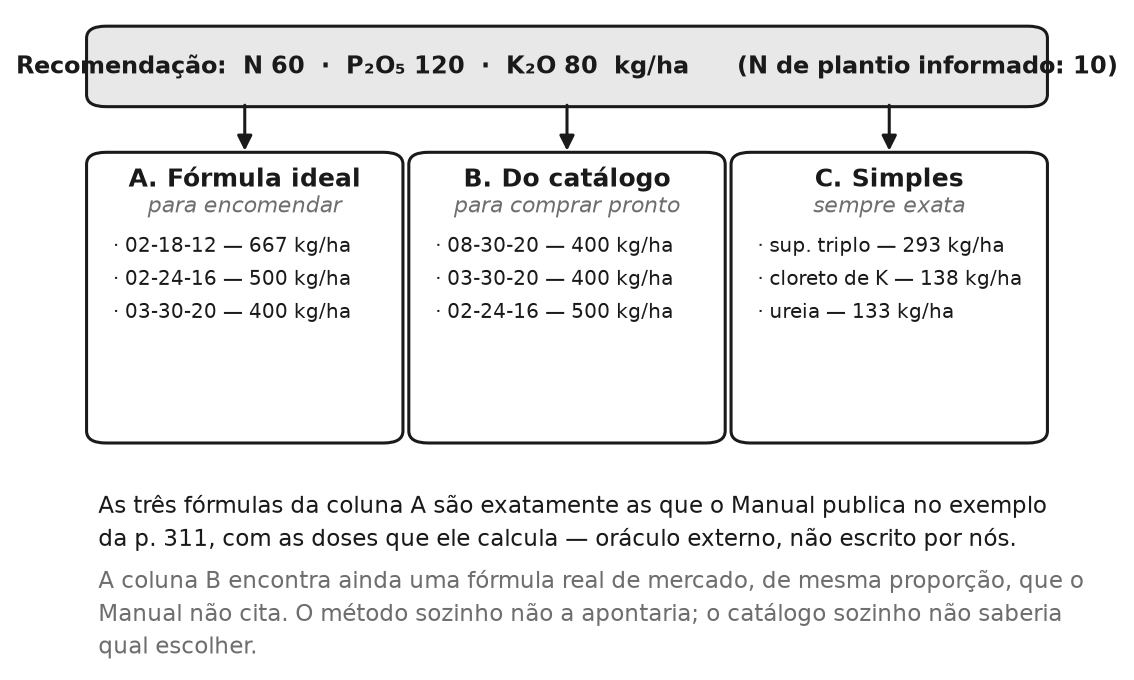
\includegraphics[width=0.95\textwidth]{fig/f4-formulacao}
\caption{Os três caminhos da formulação, resolvidos pelo próprio sistema sobre o exemplo publicado no Manual (§8.3, p.~311). A coluna A reproduz as três fórmulas e as doses que o Manual calcula. A coluna B mostra que o catálogo contém fórmulas reais de mesma proporção que o Manual não cita --- entre elas a 10-30-20, especificada em pregão público do Instituto Federal Farroupilha com entregas no Rio Grande do Sul, que vence por exigir menos massa total aplicada.}
\label{fig:formulacao}
\end{figure}

\begin{figure}[htb]
\centering
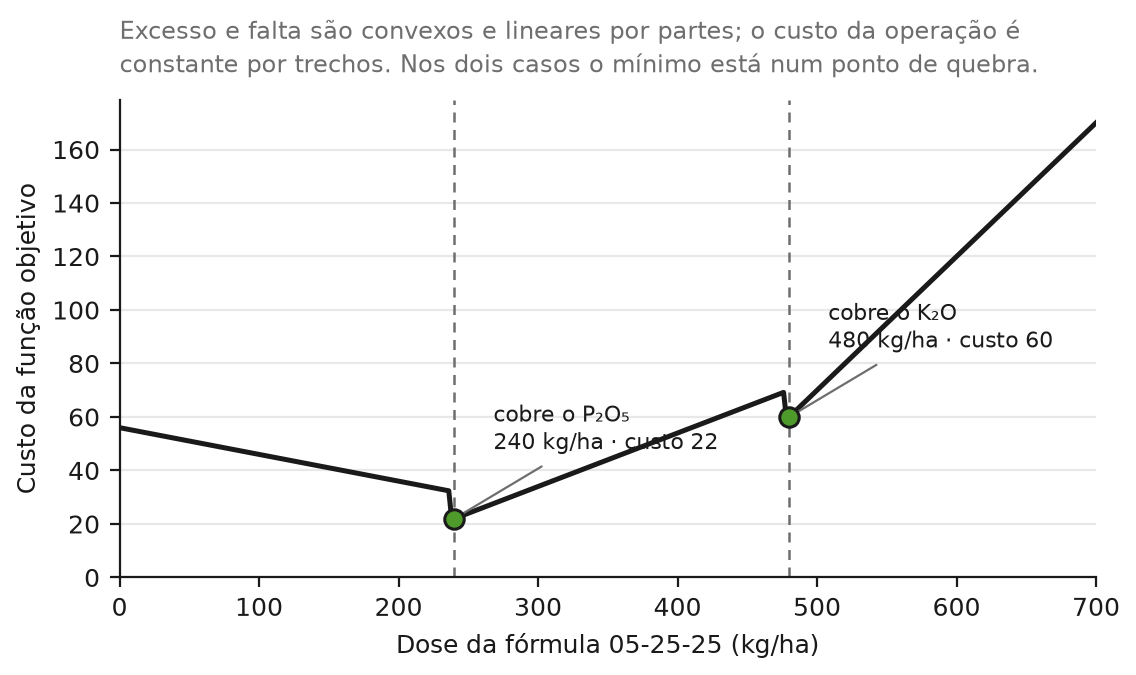
\includegraphics[width=0.95\textwidth]{fig/f5-pontos-de-quebra}
\caption{Custo em função da dose, para uma fórmula. Como o mínimo de uma função linear por partes convexa está em um ponto de quebra, basta avaliar as duas doses que atendem exatamente o P\textsubscript{2}O\textsubscript{5} e o K\textsubscript{2}O. A regra do Manual corresponde a um desses pontos.}
\label{fig:pontos-de-quebra}
\end{figure}

\subsection{Módulo de aptidão edáfica}

A estimativa de aptidão foi especificada em documento próprio --- um caderno de critérios
redigido \textbf{antes} da implementação e aprovado por escrito pelo orientador ---, sob
três princípios: nenhum limiar numérico criado pelo autor, com todo valor rastreando a
uma tabela do Manual ou a \cite{Sobral2015}; arquitetura derivada do sistema oficial, com
graus de limitação e regra do fator mínimo conforme \cite{RamalhoFilhoBeek1995} na
descrição de \cite{Hofig2015}; e toda decisão de julgamento do autor isolada, declarada
em apêndice e implementada como parâmetro configurável.

O módulo classifica a área em quatro níveis ordinais --- apta, apta com restrições,
restrita e inapta --- a partir de sete fatores de limitação, aplicando a regra do fator
mínimo. Dado ausente nunca é imputado por valor médio: gera classe indeterminada com
justificativa.

A saída traz \textbf{dois cenários}: o estado atual do solo e o estado projetado após as
correções que o próprio sistema acabou de recomendar. A diferença entre eles quantifica
o ganho atribuível à recomendação, e é o que integra os módulos --- emitir apenas um dos
dois perderia justamente a integração que distingue a solução.


\begin{figure}[htb]
\centering
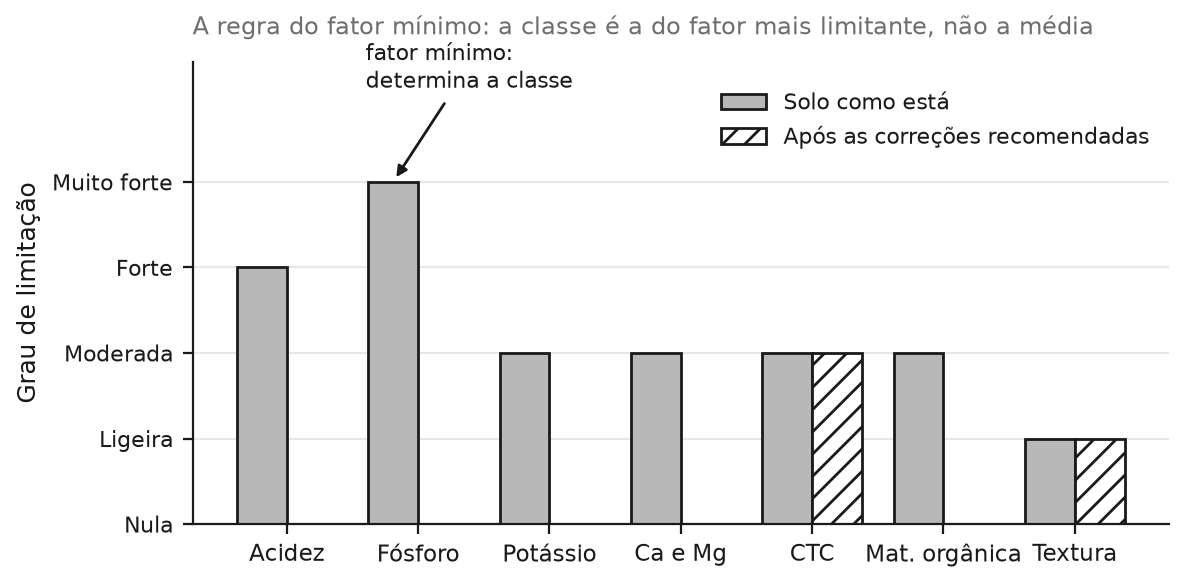
\includegraphics[width=0.95\textwidth]{fig/f6-aptidao}
\caption{Grau de limitação dos sete fatores, nos dois cenários, para uma análise real. A classe resulta do fator mais limitante, e não da média. Os fatores que a calagem e a adubação corrigem caem a zero no cenário projetado; CTC e textura permanecem, por serem limitações não corrigíveis em uma safra.}
\label{fig:aptidao}
\end{figure}

\subsection{Trilha de inferência}

Toda decisão do motor registra um passo contendo a regra aplicada, as entradas, a saída
e a fonte --- tabela e página do Manual. A trilha é impressa no laudo, agrupada por
módulo, e é o que permite a um terceiro conferir cada número sem acesso ao código. Essa
exigência é estrutural, e não opcional: em um documento que pode instruir projeto de
crédito rural, a recomendação sem procedência verificável tem pouco valor.

\section{Procedimento de avaliação}

A avaliação foi organizada em três dimensões.

\textbf{(i) Correção das saídas.} Um conjunto de casos de teste com oráculo calculado
manualmente pelo autor, a partir do Manual e sem consultar o código. Um caso é
considerado concordante quando \textbf{todas} as saídas declaradas na referência ---
necessidade de calcário e doses de N, P\textsubscript{2}O\textsubscript{5} e
K\textsubscript{2}O --- coincidem com a saída do sistema, admitida apenas tolerância de
arredondamento: uma casa decimal em t/ha para o calcário e números inteiros em kg/ha para
os nutrientes. Acertar três das quatro saídas é discordância, não acerto parcial. Apura-se
a proporção de casos concordantes, global e por grupo, com intervalo de confiança de 95\%
pelo método de \cite{Wilson1927} --- mais adequado que o intervalo normal para amostras
pequenas e proporções próximas de 1, por nunca produzir limites fora do intervalo
unitário. Casos discordantes são analisados individualmente, com a trilha de cada um.

Para a aptidão edáfica a verificação é de \textbf{conformidade}, e não de concordância:
mede se a implementação reproduz o caderno de critérios congelado, não se os critérios
estão agronomicamente corretos. O gabarito foi gerado aplicando o caderno manualmente e
é mantido em arquivo separado das entradas, de modo que o motor nunca o acessa.

\textbf{(ii) Comparação com ferramenta existente.} Natureza qualitativa, evidenciando
convergências, divergências e as funcionalidades que o SIRAS oferece e as demais não.

\textbf{(iii) Usabilidade.} Teste com usuários do público-alvo, descrito a seguir.

\subsection{Teste de usabilidade}

Participaram do teste \pendente{número final de participantes} profissionais e
estudantes do público-alvo --- agrônomos, técnicos agrícolas e estudantes concluintes de
agronomia ---, precedidos de um estudo-piloto com um participante que não integrou a
amostra.

Cada participante percorreu três roteiros em sessão única de aproximadamente 35 minutos:
(i)~demonstração conduzida pelo pesquisador sobre um cenário pronto, dando o primeiro
contato; (ii)~cenário fechado, entregue em ficha, executado pelo participante
\textbf{sozinho}; e (iii)~geração de um laudo \textbf{livre}, com cultura e dados de
escolha do próprio participante. Em (ii) e (iii) o pesquisador não auxiliou, devolvendo
as perguntas ao participante, pois cada intervenção suprimiria o registro de um problema
de usabilidade.

Concluída a sessão, e em momento separado, o participante respondeu a um
\textbf{questionário pós-teste estruturado pelas dez heurísticas de Nielsen}
\citep{Nielsen1994}, atribuindo a cada heurística uma nota de severidade de 0 a 4 e
descrevendo em texto livre as falhas e as telas em que ocorreram, seguido de quatro
perguntas abertas. Adotou-se esse instrumento em lugar do \textit{System Usability Scale}
\citep{Brooke1996} porque o SUS produz um escore único, ao passo que esta etapa precisava
produzir um diagnóstico acionável: a grade das heurísticas classifica cada problema pela
dimensão que ele viola e permite ordenar as correções por severidade. Perde-se a
comparabilidade com a literatura de escores SUS, o que se registra como limitação.

Cabe a distinção terminológica: \textbf{não se trata de avaliação heurística} no sentido
de \cite{NielsenMolich1990}, que designa a inspeção por especialistas em usabilidade,
sem usuários e sem tarefas. São usuários finais executando tarefas reais, e as notas ---
atribuídas por usuários a heurísticas, e não por avaliadores a problemas --- exprimem
percepção de gravidade, analisada por estatística descritiva, sem inferência. O
dimensionamento da amostra seguiu \cite{NielsenLandauer1993}.

A versão avaliada foi congelada antes da primeira sessão e mantida inalterada até a
última, de modo que todos os participantes avaliassem o mesmo sistema. Problemas
identificados durante a coleta foram anotados, não corrigidos. A etapa não requer
submissão a comitê de ética, e não houve termo de consentimento assinado: o participante
usou o sistema e respondeu ao formulário, que não coleta identificação direta.

% Resultados e Discussão — a seção principal do artigo.
%
% REGRA QUE VALE AQUI ACIMA DE TUDO: nada é escrito antes de ser medido. Onde o dado
% ainda não existe há \pendente{}, em vermelho, dizendo o que falta e de onde virá.
% Antes de entregar, compilar e conferir que não sobrou nenhum marcador.
%
% ESTADO EM 10/10/2026:
%   4.1 Cobertura funcional ......... ESCRITO (medido)
%   4.2 Correção das saídas ......... ESCRITO (medido, 10/10/2026)
%   4.3 Conformidade da aptidão ..... ESCRITO (medido)
%   4.4 Comparação com FertFacil .... PENDENTE (depende da execução da comparação)
%   4.5 Usabilidade ................. PENDENTE (depende da coleta, 20/10 a 14/11)
%   4.6 Discussão geral ............. PARCIAL (fecha quando 4.4 e 4.5 existirem)
%
% Os números de 4.1 a 4.3 são reproduzíveis: saem de
%   python scripts/gera_tabela_concordancia.py
%   python -m pytest --completa

\chapter{Resultados e Discussão}\label{chap:resultados}

\section{Cobertura funcional e verificação técnica}

O sistema cobre as 61 culturas e grupos de culturas do escopo, com os quatro módulos ---
calagem, adubação, indicação de adubo formulado e aptidão edáfica --- operando para
todas elas. A verificação técnica foi conduzida por uma bancada automatizada que percorre
as 61 culturas contra 10 perfis de solo distintos, exercitando cada estado que a interface
oferece.

Dos estados verificados, 340 produziram laudo completo; 22 foram recusados nomeando o
campo que a fase da cultura exige e não fora informado; e 5 foram recusados por limite
declarado de implementação. \textbf{Nenhum derrubou a aplicação.} A distinção importa: a
recusa explicada é comportamento projetado --- o sistema diz o que falta e por quê ---,
enquanto a falha não tratada seria defeito. As cinco combinações recusadas por limite
correspondem a três frutíferas cuja adubação de manutenção o Manual define por teor
foliar, sem correspondência publicada com o teor do solo; são, portanto, limite da fonte
e não da implementação.

A suíte de testes conta 4.951 casos automatizados, todos passando, organizados em duas
camadas: uma rápida, para execução a cada alteração, e uma completa, que acrescenta as
bancadas de maior volume. Além dela, dois verificadores independentes são executados: a
validação de todos os arquivos da base contra os respectivos \textit{JSON Schema}, e a
reprodução das 32 classificações de fósforo e potássio publicadas no Anexo~1 do Manual,
que funciona como \textbf{oráculo externo} --- os valores de entrada e as classes
resultantes são do próprio Manual, não do autor. Nessa verificação houve 0 divergências
em 32 classificações.

\section{Correção das recomendações}

A \cref{tab:concordancia} apresenta a concordância entre as saídas do sistema e o oráculo
calculado manualmente pelo autor.

\begin{table}[htb]
\centering
\caption{Concordância das recomendações com o oráculo, por grupo de cultura}
\label{tab:concordancia}
\begin{tabular}{lrrrr}
\toprule
\textbf{Grupo} & \textbf{Casos} & \textbf{Concordantes} & \textbf{Taxa} & \textbf{IC 95\% (Wilson)} \\
\midrule
Grãos        &  9 &  9 & 100,0\% & [70,1\%; 100,0\%] \\
Frutíferas   &  4 &  4 & 100,0\% & [51,0\%; 100,0\%] \\
Erva-mate    &  2 &  2 & 100,0\% & [34,2\%; 100,0\%] \\
\midrule
\textbf{Global} & \textbf{15} & \textbf{15} & \textbf{100,0\%} & \textbf{[79,6\%; 100,0\%]} \\
\bottomrule
\end{tabular}
\end{table}


\begin{figure}[htb]
\centering
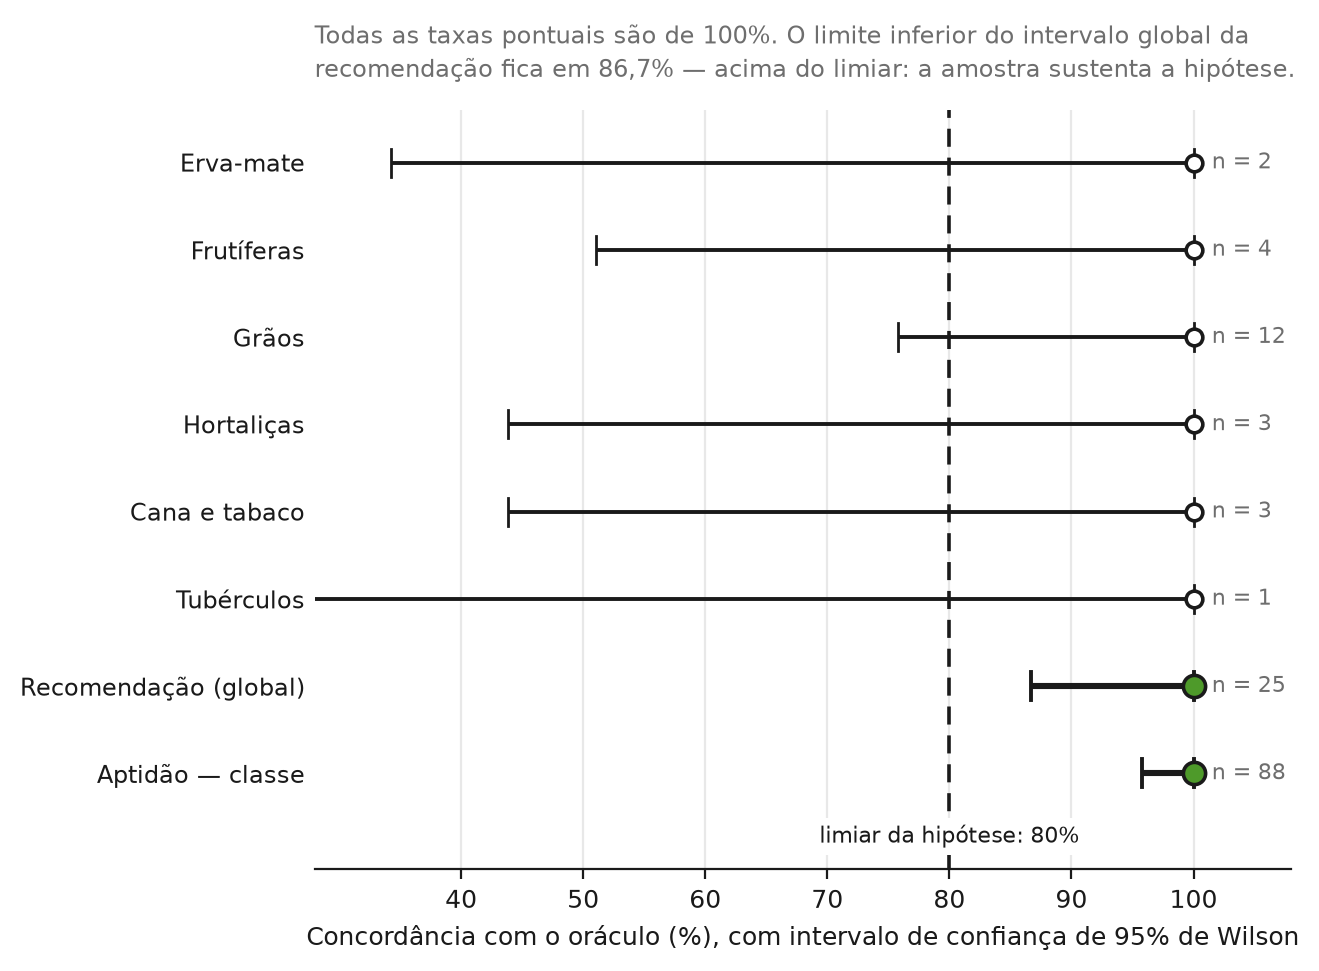
\includegraphics[width=0.95\textwidth]{fig/f7-concordancia}
\caption{Concordância com o oráculo, por grupo e global, com intervalo de confiança de 95\% de Wilson. Todas as taxas pontuais são de 100\%; o que o intervalo mostra é o efeito do tamanho da amostra, e o limite inferior do intervalo global da recomendação fica abaixo do limiar de 80\% que a hipótese estabelece.}
\label{fig:concordancia}
\end{figure}

Não houve caso discordante. Toda necessidade de calcário e toda dose de nitrogênio,
fósforo e potássio coincidiram com o valor calculado à mão, dentro da tolerância de
arredondamento declarada.

\textbf{O resultado precisa ser lido com a ressalva que ele próprio impõe.} Com 15 casos
e concordância integral, o limite inferior do intervalo de confiança de 95\% situa-se em
\textbf{79,6\%} --- isto é, \textbf{abaixo} do patamar de 80\% que a hipótese
H\textsubscript{1.1} estabelece. O resultado pontual satisfaz o critério; o intervalo,
por margem estreita, não. A causa não é erro do sistema, que acertou todos os casos, mas
o tamanho da amostra: com concordância integral, 16 casos elevariam o limite inferior a
80,6\% e 20 casos a 83,9\%.

\pendente{se mais casos forem calculados até a entrega, atualizar a tabela rodando
\texttt{python scripts/gera\_tabela\_concordancia.py} e reescrever este parágrafo com o
intervalo novo}

Duas observações sobre a natureza dessa evidência. A primeira é que o conjunto ficou
abaixo do alvo de 40 a 80 casos declarado no protocolo de validação, por restrição de
tempo: cada caso exige cálculo manual completo a partir do Manual, incluindo memória de
cálculo, e é esse custo que limita o conjunto. A segunda, e mais importante, é o
\textbf{risco de circularidade}: o sistema foi construído a partir do Manual e a
referência é o Manual aplicado pelo mesmo autor, de modo que o que se mede é a fidelidade
da implementação à transcrição --- não a adequação agronômica dos critérios. A mitigação
prevista é a incorporação de casos oriundos de laudos reais, com recomendação elaborada
por profissional habilitado, e o verificador do Anexo~1 citado na seção anterior é o
único oráculo hoje genuinamente externo.

\section{Conformidade do módulo de aptidão edáfica}

Para a aptidão, a verificação é de conformidade: mede se a implementação reproduz o
caderno de critérios aprovado, não se os critérios estão corretos. O conjunto tem 88
casos gabaritados, com o gabarito mantido em arquivo separado das entradas e gerado pela
aplicação manual da especificação, sem consulta ao código.

O resultado foi de \textbf{88/88 = 100\%} tanto na classe de aptidão atribuída quanto no
fator determinante, com intervalo de confiança de 95\% de [95,8\%; 100,0\%]. Conferir
também o fator determinante, e não apenas a classe, é o que impede que um acerto de
classe pelo motivo errado passe despercebido.

A ordem cronológica sustenta a alegação de não circularidade: a especificação foi
redigida e aprovada \textbf{antes} da implementação do motor, e o gabarito foi derivado
dela, não do código. Ao longo do desenvolvimento foram registradas oito divergências de
conformidade, todas analisadas individualmente e documentadas. Vale o registro de que
\textbf{nenhuma delas exigiu alterar um critério}: quatro eram lacunas de transcrição da
base, uma era erro de geração do gabarito, duas eram inconsistências de derivação entre
módulos --- resolvidas fazendo os dois derivarem da mesma grandeza, sem mudar limiar ---
e uma era defeito de arredondamento prematuro.

Convém, porém, não apresentar os dois "100\%" como se pesassem igual. A conformidade da
aptidão apoia-se em 88 casos e verifica a implementação contra uma especificação própria;
a concordância das recomendações apoia-se em 15 casos e verifica contra o Manual. A
segunda é a afirmação mais forte e a de evidência mais estreita.

\section{Comparação com ferramenta existente}

\pendente{executar a comparação com o FertFacil sobre um subconjunto dos casos e
escrever esta seção: convergências, divergências e sua explicação (diferença de critério
ou de edição do Manual), e as funcionalidades que o SIRAS oferece e a ferramenta
comparada não --- em especial a aptidão edáfica integrada e a trilha de inferência}

\section{Avaliação de usabilidade}

\pendente{seção inteira --- depende da coleta prevista para 20/10 a 14/11/2026. Rodar
\texttt{python scripts/consolidar\_heuristicas.py} sobre o CSV exportado do formulário e
escrever a partir da saída dele}

A seção deverá apresentar, nesta ordem: o perfil da amostra, a partir das perguntas de
caracterização do formulário; a conclusão das tarefas em cada roteiro; a tabela de
severidade por heurística, com média, mediana, mínimo e máximo; a lista de problemas
priorizada pela severidade; e a síntese das respostas abertas.

\pendente{perfil da amostra}
\pendente{conclusão das tarefas por roteiro}
\pendente{figura de severidade por heurística --- rodar
\texttt{scripts/consolidar\_heuristicas.py} sobre o CSV do formulário e depois
\texttt{scripts/gerar\_figuras\_artigo.py}, que só então produz
\texttt{fig/f8-usabilidade.png}. Inserir aqui com \texttt{label=fig:usabilidade}}
\pendente{lista priorizada de problemas, e quais foram corrigidos antes da entrega}
\pendente{síntese das quatro perguntas abertas, separando o juízo sobre a ferramenta do
juízo sobre a recomendação agronômica}

Na discussão desta seção, declarar as ameaças à validade já identificadas: o pesquisador
é o autor do sistema, o que tende a suavizar a crítica --- mitigado por responder o
questionário fora da sessão e sem a presença dele; o primeiro roteiro treina o
participante, de modo que o que se mede é adoção assistida, e não descoberta autônoma; e
a escala de severidade, atribuída por usuários a heurísticas em vez de por avaliadores a
problemas, exprime percepção de gravidade e não gravidade técnica.

\section{Discussão}

Os resultados disponíveis sustentam que a automatização dos critérios do Manual é
viável e que a implementação os reproduz com fidelidade: concordância integral nos casos
com oráculo, conformidade integral na aptidão e nenhuma falha não tratada em 367 estados
exercitados.

O diferencial declarado na introdução --- integrar recomendação de manejo e estimativa de
aptidão a partir de uma análise individual --- materializou-se na emissão conjunta dos
dois cenários de aptidão, atual e projetado, em que a diferença entre eles quantifica o
ganho atribuível à recomendação emitida. Nenhuma das ferramentas levantadas no
\cref{chap:revisao} produz essa saída.

Um resultado colateral merece registro por ilustrar o que a combinação de método
normativo e catálogo de mercado permite. Para a recomendação usada como exemplo pelo
próprio Manual, o sistema reproduz as três fórmulas que ele indica, com as doses
publicadas, e encontra ainda uma quarta --- de mesma proporção e igualmente exata ---
que consta de levantamento de fórmulas efetivamente utilizadas por produtores do Sul.
O método, sozinho, não a apontaria; o catálogo, sozinho, não saberia qual escolher.

As limitações mais relevantes são três, e nenhuma é contornável por esforço de
implementação. A primeira é a \textbf{circularidade parcial} da validação, já discutida.
A segunda é que a estimativa de aptidão é \textbf{exclusivamente edáfica}, sem relevo,
clima, drenagem ou suscetibilidade à erosão --- o que o próprio Manual indica como
necessário a uma avaliação de aptidão agrícola. A terceira é que a indicação de adubo
formulado faz um ranking \textbf{nutricional}, e não de custo: o Manual recomenda
escolher pelo menor custo por unidade de NPK, e o sistema não dispõe de preços, que são
do comprador e variam por revenda e por semana.

\pendente{fechar a discussão depois das seções 4.4 e 4.5, retomando o que a comparação
com a ferramenta existente e o teste com usuários acrescentaram}

% Conclusão — alvo: 3 a 4 parágrafos (orientador, 10/10/2026).
% Retoma o objetivo, diz em que medida foi alcançado, destaca a contribuição principal,
% os resultados e as limitações mais relevantes, e fecha com trabalhos futuros.
%
% ESTADO: rascunho. Os parágrafos 1, 3 e 4 estão escritos sobre o que já foi medido; o
% parágrafo 2 depende da usabilidade e da comparação, e por isso está marcado. Reescrever
% o conjunto depois que o capítulo 4 fechar — a conclusão é a última coisa a ser redigida.

\chapter{Conclusão}\label{chap:conclusao}

Este trabalho teve por objetivo desenvolver e avaliar o SIRAS, um sistema especialista
baseado em regras para interpretação de análises de solo, recomendação de calagem e
adubação e estimativa de aptidão edáfica, segundo os critérios do Manual de Calagem e
Adubação para os estados do RS e de SC. O objetivo foi alcançado no que diz respeito à
construção e à verificação do artefato: o sistema cobre as 61 culturas e grupos de
culturas do escopo, emite recomendação e estimativa de aptidão a partir de uma única
análise, e cada número do laudo é acompanhado da regra, da tabela e da página que o
produziram. Nos casos com oráculo calculado manualmente, a concordância foi integral; na
conformidade do módulo de aptidão frente à especificação aprovada antes da
implementação, também.

A contribuição principal não está em automatizar a recomendação --- isso ferramentas
existentes já fazem, e bem ---, mas em \textbf{integrar}, a partir de uma análise
individual de solo, a recomendação de manejo e a estimativa de aptidão da cultura
escolhida, emitindo os dois cenários de solo, o atual e o projetado após as correções
recomendadas, de modo que a diferença entre eles quantifique o ganho atribuível à
própria recomendação. Soma-se a isso a rastreabilidade integral das saídas e a separação
explícita, no próprio sistema, entre o que é norma, o que é legislação, o que é convenção
comercial e o que é dado de fabricante --- distinção que, no domínio tratado, costuma se
perder.

\pendente{parágrafo sobre o que o teste de usabilidade e a comparação com a ferramenta
existente mostraram --- escrever depois das seções 4.4 e 4.5}

As limitações mais relevantes são de três ordens. A validação apoia-se em um conjunto de
casos menor do que o planejado e cuja referência foi calculada pelo mesmo autor que
implementou o sistema, de modo que ela mede a fidelidade da implementação aos critérios
transcritos, e não a adequação agronômica desses critérios; o intervalo de confiança
obtido reflete esse tamanho de amostra. A estimativa de aptidão é exclusivamente
edáfica, sem relevo, clima nem drenagem, e por isso não substitui uma avaliação de
aptidão agrícola das terras. E a indicação de adubo formulado ordena as alternativas por
adequação nutricional, não por custo, porque o sistema não dispõe de preços.

Como trabalhos futuros, três encaminhamentos se destacam. O primeiro é ampliar o
conjunto de casos de validação com \textbf{laudos reais anonimizados}, cuja recomendação
tenha sido elaborada por profissional habilitado --- o que substituiria o oráculo do
próprio autor por referência independente e romperia a circularidade parcial que hoje
limita a força da evidência. O segundo é incorporar à estimativa de aptidão os fatores
de ambiente que ela hoje não considera, aproximando-a do sistema de avaliação de aptidão
agrícola sem abandonar a escala individual da propriedade. O terceiro é a implantação em
servidor remoto, com persistência do histórico de análises por propriedade, o que
permitiria acompanhar a evolução da fertilidade ao longo das safras --- informação que
uma análise isolada não oferece e que é central ao planejamento de longo prazo.


%----------------------------------------------------------------
% Referências bibliográficas
%----------------------------------------------------------------
\renewcommand*{\bibname}{\capbib}
\clearpage\phantomsection\addcontentsline{toc}{chapter}{\MakeUppercase{\capbib}}
\bibliography{referencias}

\end{document}
